\vspace{0.2cm}

\section{Proposed Transformation}
\label{sec:proposed}

\subsection{Overview}

We demonstrate the proposed transformation using the circuit in
\Cref{fig_transformation}A as a working example. The circuit is a~handshake
decoupling element (an S-element \cite{bardsley2000implementing}) and its
state is given by nets \texttt{ao}, \texttt{ri}, \texttt{ai}, \texttt{ro} and
the output of gate \texttt{g0}. In a conventional synchronous simulator, the
circuit is treated as combinational logic and all of its nets are evaluated on
each cycle. This does not allow individual transitions, their possible
orderings or their timings with respect to the environment to be simulated. To
capture these behavioral mechanics, we insert flip-flops at the outputs of all
non-zero delay gates and use a~vector of enable signals (\texttt{en}) to
select which net is updated on each cycle. We~prevent multiple transitions
from firing during the same cycle by constraining \texttt{en} such that no
more than a single bit is active at time. However, we allow all \texttt{en}
bits to be inactive to simulate stall cycles in which no transitions occur
(this is necessary for deadlock freeness checking, and is discussed in more
details in Subsection~\ref{subsec:deadlock_freeness}).

To use the created synchronous model in a simulation, inputs must be provided
in accordance with circuit's specification (or better yet, generated by an
actual implementation of the circuit's environment), and a sequence of
\texttt{en} vectors must be supplied to determine transition ordering. While
there could be more than a single valid \texttt{en} sequence (and supplying
these by hand may be laborious) the model is primarily intended for formal
verification and so our focus is to enable it to capture all possible forms of
behavior. The task of generating \texttt{en} sequences and exploring the
resulting circuit behavior will be left to formal tools.

% fig_compliance

\begin{figure*}[!t]
\begin{center}

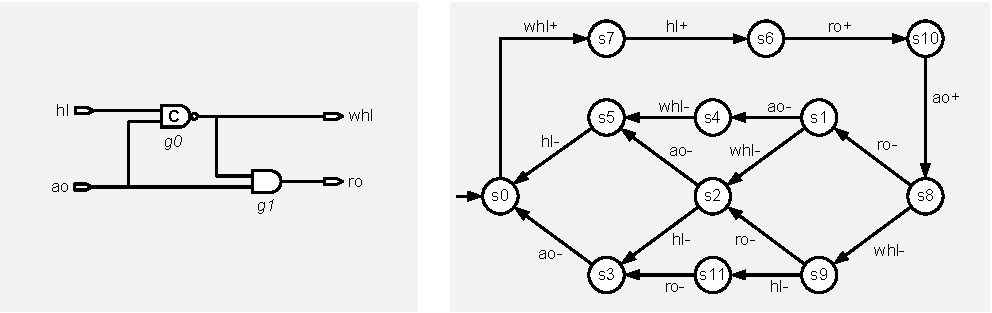
\includegraphics[width=17cm]{figures/fig_compliance}

\caption{
Example asynchronous circuit (left) and its specification as a state graph (right)
}

\label{fig_compliance}
\end{center}

\end{figure*}


Some gates such as C-elements are capable of retaining their own state and are
therefore handled differently by the transformation. They are replaced with
clocked equivalents and no flip-flops are inserted at their outputs. The
clocked equivalents have an enable input which is connected to the
corresponding bit from the enable vector \texttt{en}. An example of this
special case handling is gate \texttt{g0} in \Cref{fig_transformation}.

\subsection{Applying the Transformation}

We created a tool that applies the described transformation to asynchronous
circuits netlists such as the ones synthesized by Petrify
\cite{cortadella1997petrify}. While there are no reasons preventing the
transformation from being performed by hand correctly, the ability to automate
it has two important practical implications. First, it avoids manual
translation errors that may introduce differences between circuit and model
behavior (essentially the same risk with model faithfulness that system-level
verification is intended to avoid). Second, it enables the transformation to
be integrated seamlessly into existing design flows, remaining transparent to
the designer and not affecting other tools in the flow (we present a use case
verification flow demonstrating this practically in \Cref{subsec:mixed}).
Another important practical consideration is that the vector~\texttt{en} can
be declared as an internal unbound register instead of being added to the
circuit as an input. This way the original circuit and the generated model
will have identical interfaces, allowing the model to be used as a drop-in
replacement for the circuit.
